\documentclass[12pt,a4paper]{article}
\title{Lab9-OpenCV}
\usepackage{ctex}
\usepackage{amsmath,amscd,amsbsy,amssymb,latexsym,url,bm,amsthm}
\usepackage{epsfig,graphicx,subfigure}
\usepackage{enumitem,balance}
\usepackage{wrapfig}
\usepackage{mathrsfs,euscript}
\usepackage[usenames]{xcolor}
\usepackage{hyperref}
\usepackage[vlined,ruled,commentsnumbered,linesnumbered]{algorithm2e}
\usepackage{float}
\usepackage{geometry}
\usepackage{listings}
\geometry{a4paper,scale=0.8}
\usepackage[T1]{fontenc}
\usepackage[utf8]{inputenc}
\usepackage{amssymb}
\usepackage{graphicx}
\usepackage{subfigure}
% --- Python code template ---
\usepackage[utf8]{inputenc}
% Default fixed font does not support bold face
\DeclareFixedFont{\ttb}{T1}{txtt}{bx}{n}{12} % for bold
\DeclareFixedFont{\ttm}{T1}{txtt}{m}{n}{12}  % for normal

% Custom colors
\usepackage{color}
\definecolor{deepblue}{rgb}{0,0,0.5}
\definecolor{deepred}{rgb}{0.6,0,0}
\definecolor{deepgreen}{rgb}{0,0.5,0}

\usepackage{listings}

% Python style for highlighting
\newcommand\pythonstyle{\lstset{
language=Python,
basicstyle=\ttm,
morekeywords={self},              % Add keywords here
keywordstyle=\ttb\color{deepblue},
emph={MyClass,__init__},          % Custom highlighting
emphstyle=\ttb\color{deepred},    % Custom highlighting style
stringstyle=\color{deepgreen},
frame=tb,                         % Any extra options here
showstringspaces=false
}}
% Python environment
\lstnewenvironment{python}[1][]
{
\pythonstyle
\lstset{#1}
}
{}

% Python for external files
\newcommand\pythonexternal[2][]{{
\pythonstyle
\lstinputlisting[#1]{#2}}}

% Python for inline
\newcommand\pythoninline[1]{{\pythonstyle\lstinline!#1!}}

% --- Python code template ---


% --- HTML lstlisting template --- %
\makeatletter
\usepackage{color}
\definecolor{lightgray}{rgb}{0.95, 0.95, 0.95}
\definecolor{darkgray}{rgb}{0.4, 0.4, 0.4}
%\definecolor{purple}{rgb}{0.65, 0.12, 0.82}
\definecolor{editorGray}{rgb}{0.95, 0.95, 0.95}
\definecolor{editorOcher}{rgb}{1, 0.5, 0} % #FF7F00 -> rgb(239, 169, 0)
\definecolor{editorGreen}{rgb}{0, 0.5, 0} % #007C00 -> rgb(0, 124, 0)
\definecolor{orange}{rgb}{1,0.45,0.13}		
\definecolor{olive}{rgb}{0.17,0.59,0.20}
\definecolor{brown}{rgb}{0.69,0.31,0.31}
\definecolor{purple}{rgb}{0.38,0.18,0.81}
\definecolor{lightblue}{rgb}{0.1,0.57,0.7}
\definecolor{lightred}{rgb}{1,0.4,0.5}
\usepackage{upquote}
\usepackage{listings}
% CSS
\lstdefinelanguage{CSS}{
  keywords={color,background-image:,margin,padding,font,weight,display,position,top,left,right,bottom,list,style,border,size,white,space,min,width, transition:, transform:, transition-property, transition-duration, transition-timing-function},	
  sensitive=true,
  morecomment=[l]{//},
  morecomment=[s]{/*}{*/},
  morestring=[b]',
  morestring=[b]",
  alsoletter={:},
  alsodigit={-}
}

% JavaScript
\lstdefinelanguage{JavaScript}{
  morekeywords={typeof, new, true, false, catch, function, return, null, catch, switch, var, if, in, while, do, else, case, break},
  morecomment=[s]{/*}{*/},
  morecomment=[l]//,
  morestring=[b]",
  morestring=[b]'
}

\lstdefinelanguage{HTML5}{
  language=html,
  sensitive=true,	
  alsoletter={<>=-},	
  morecomment=[s]{<!-}{-->},
  tag=[s],
  otherkeywords={
  % General
  >,
  % Standard tags
	<!DOCTYPE,
  </html, <html, <head, <title, </title, <style, </style, <link, </head, <meta, />,
	% body
	</body, <body,
	% Divs
	</div, <div, </div>, 
	% Paragraphs
	</p, <p, </p>,
	% scripts
	</script, <script,
  % More tags...
  <canvas, /canvas>, <svg, <rect, <animateTransform, </rect>, </svg>, <video, <source, <iframe, </iframe>, </video>, <image, </image>, <header, </header, <article, </article
  },
  ndkeywords={
  % General
  =,
  % HTML attributes
  charset=, src=, id=, width=, height=, style=, type=, rel=, href=,
  % SVG attributes
  fill=, attributeName=, begin=, dur=, from=, to=, poster=, controls=, x=, y=, repeatCount=, xlink:href=,
  % properties
  margin:, padding:, background-image:, border:, top:, left:, position:, width:, height:, margin-top:, margin-bottom:, font-size:, line-height:,
	% CSS3 properties
  transform:, -moz-transform:, -webkit-transform:,
  animation:, -webkit-animation:,
  transition:,  transition-duration:, transition-property:, transition-timing-function:,
  }
}

\lstdefinestyle{htmlcssjs} {%
  % General design
%  backgroundcolor=\color{editorGray},
  basicstyle={\footnotesize\ttfamily},   
  frame=b,
  % line-numbers
  xleftmargin={0.75cm},
  numbers=left,
  stepnumber=1,
  firstnumber=1,
  numberfirstline=true,	
  % Code design
  identifierstyle=\color{black},
  keywordstyle=\color{blue}\bfseries,
  ndkeywordstyle=\color{editorGreen}\bfseries,
  stringstyle=\color{editorOcher}\ttfamily,
  commentstyle=\color{brown}\ttfamily,
  % Code
  language=HTML5,
  alsolanguage=JavaScript,
  alsodigit={.:;},	
  tabsize=2,
  showtabs=false,
  showspaces=false,
  showstringspaces=false,
  extendedchars=true,
  breaklines=true,
  % German umlauts
  literate=%
  {Ö}{{\"O}}1
  {Ä}{{\"A}}1
  {Ü}{{\"U}}1
  {ß}{{\ss}}1
  {ü}{{\"u}}1
  {ä}{{\"a}}1
  {ö}{{\"o}}1
}
%
\lstdefinestyle{py} {%
language=python,
literate=%
*{0}{{{\color{lightred}0}}}1
{1}{{{\color{lightred}1}}}1
{2}{{{\color{lightred}2}}}1
{3}{{{\color{lightred}3}}}1
{4}{{{\color{lightred}4}}}1
{5}{{{\color{lightred}5}}}1
{6}{{{\color{lightred}6}}}1
{7}{{{\color{lightred}7}}}1
{8}{{{\color{lightred}8}}}1
{9}{{{\color{lightred}9}}}1,
basicstyle=\footnotesize\ttfamily, % Standardschrift
numbers=left,               % Ort der Zeilennummern
%numberstyle=\tiny,          % Stil der Zeilennummern
%stepnumber=2,               % Abstand zwischen den Zeilennummern
numbersep=5pt,              % Abstand der Nummern zum Text
tabsize=4,                  % Groesse von Tabs
extendedchars=true,         %
breaklines=true,            % Zeilen werden Umgebrochen
keywordstyle=\color{blue}\bfseries,
frame=b,
commentstyle=\color{brown}\itshape,
stringstyle=\color{editorOcher}\ttfamily, % Farbe der String
showspaces=false,           % Leerzeichen anzeigen ?
showtabs=false,             % Tabs anzeigen ?
xleftmargin=17pt,
framexleftmargin=17pt,
framexrightmargin=5pt,
framexbottommargin=4pt,
%backgroundcolor=\color{lightgray},
showstringspaces=false,      % Leerzeichen in Strings anzeigen ?
}%
%
\makeatother

%\begin{lstlisting}[style=htmlcssjs]
% --- HTML lstlisting template --- %


















\title{Lab14\quad LSH}
\date{2021.12}
\author{孙济宸\quad \quad 学号:520030910016 \quad  \quad 班级:F2003003}
\begin{document}
\maketitle
\section{实验概览}
\begin{enumerate}
\item 实现LSH,通过颜色直方图特征哈希,进行图片分类和检索
\end{enumerate}
\section{实验环境}
\begin{itemize}
	\item numpy
	\item cv2 (读写图片)
	\item colorHist (lab9颜色直方图)

\end{itemize}
\newpage

\section{练习题的解决思路}
首先将图片分为4块,计算每块子图的RGB直方图,均分到[0,1,2]上,得到12维特征向量;
\begin{lstlisting}[style=py]
	quadrants = [((0,0),(H//2, W//2)) , ((0, W//2), (H//2, W)),
                 ((H//2,0), (H, W//2)), ((H//2, W//2), (H, W))]    
    # divide into 4 sections
    feat = []
    for sect in quadrants:
        c1, c2 = sect
        #print(c1, c2)
        sub_img = img[c1[0]:c2[0], c1[1]:c2[1]] 
        rgb = colorHist.RGB_hist(sub_img)
        
        rgbf = np.digitize(rgb, [0, 0.3, 0.6]) - 1     # 按照0~0.3, 0.3~0.6, 0.6~1 分类
        #print(rgbf)
        feat += list(rgbf)
\end{lstlisting}

接着计算Hamming码:
$$v(p)=Unary_c({p_1}) \dots Unary_c({p_d})$$
这里$C = 2, d = 12$
接着把Hammming码投影到集合
$$I = \{i_1, i_2, \dots i_m \}$$上
投影$g(p)=p_{i_1}p_{i_2}\dots p_{i_m}$,其中$p_{i_j}$是$v(p)$的第${i_j}$个元素
\begin{lstlisting}[style=py]
def hamming(p, d, C):
    hcode = []
    for p_i in p:
        hcode += [1] * int(p_i)
        hcode += [0] * int(C - p_i)
    return hcode

# bitwise projection 
def projection(set1, set2): 
    proj = [set1[x] for x in set2]
    return proj
\end{lstlisting}

这样一张图片就可以用$m$维哈希值表示。根据LSH的理论,相似的图片会有相近的哈希值(向量)。
对于target和dataset中的图片,计算出每张图的哈希向量,再计算向量的相似度(本实验中用标准化后的点乘),就可以完成图片检索。

\section{代码运行结果}
\subsection{I=\{3,4,5,6,11,12\}}
\begin{figure}[H]
\subfigure[target]{
\centering	
	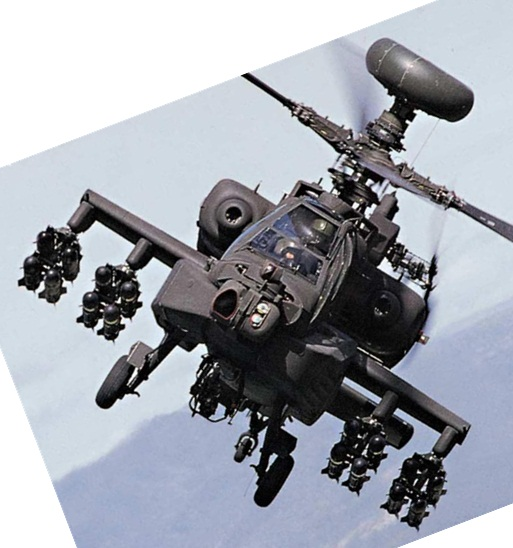
\includegraphics[width=0.3\textwidth]{../target.jpg}
	
}
\subfigure[]{
	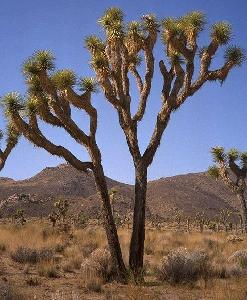
\includegraphics[width=0.3\textwidth]{../match_top_1.png}
	\centering
}
\subfigure[]{
	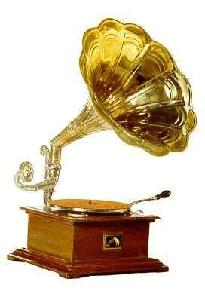
\includegraphics[width=0.3\textwidth]{../match_top_2.png}
	\centering
}
\subfigure[]{
	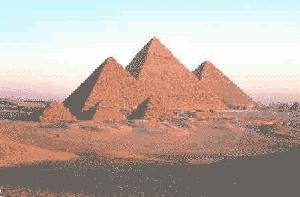
\includegraphics[width=0.3\textwidth]{../match_top_3.png}
	
	\centering
}
\subfigure[]{
	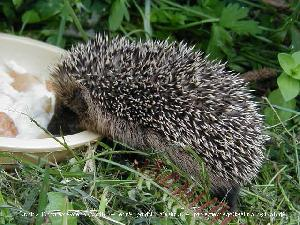
\includegraphics[width=0.3\textwidth]{../match_top_4.png}
	\centering
}
\subfigure[]{
	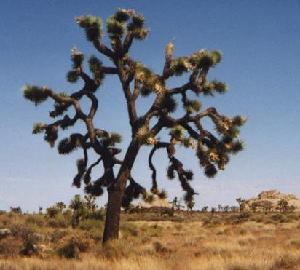
\includegraphics[width=0.3\textwidth]{../match_top_5.png}
	\centering
}
	\caption{LSH匹配}
	\centering
\end{figure}


\subsection{I=\{4,8,12,16\}}
\begin{figure}[H]
\subfigure[target]{
\centering	
	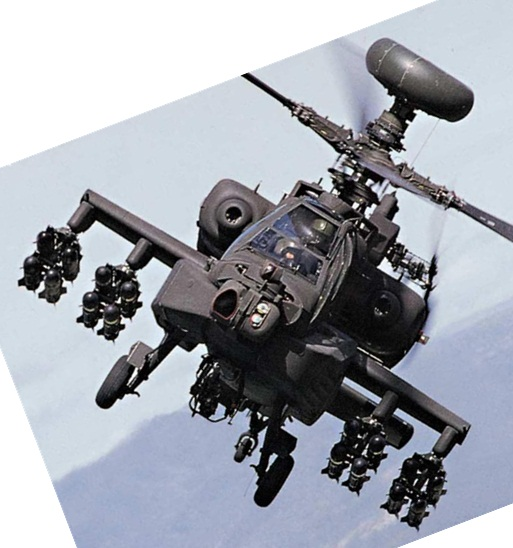
\includegraphics[width=0.3\textwidth]{../target.jpg}
	
}
\subfigure[]{
	\includegraphics[width=0.3\textwidth]{../match_top_1_{3, 4, 5, 6, 11, 12}}
	\centering
}
\subfigure[]{
	\includegraphics[width=0.3\textwidth]{../match_top_2_{3, 4, 5, 6, 11, 12}}
	\centering
}
\subfigure[]{
	\includegraphics[width=0.3\textwidth]{../match_top_3_{3, 4, 5, 6, 11, 12}}
	
	\centering
}
\subfigure[]{
	\includegraphics[width=0.3\textwidth]{../match_top_4_{3, 4, 5, 6, 11, 12}}
	\centering
}
\subfigure[]{
	\includegraphics[width=0.3\textwidth]{../match_top_5_{3, 4, 5, 6, 11, 12}}
	\centering
}
	\caption{LSH匹配}
	\centering
\end{figure}

\subsection{I=\{5, 7, 9, 11\}}
\begin{figure}[H]
\subfigure[target]{
\centering	
	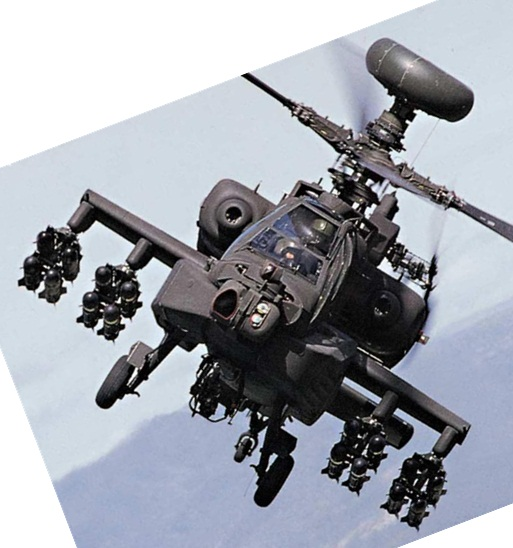
\includegraphics[width=0.3\textwidth]{../target.jpg}
	
}
\subfigure[]{
	\includegraphics[width=0.3\textwidth]{../match_top_1_[5, 7, 9, 11].png}
	\centering
}
\subfigure[]{
	\includegraphics[width=0.3\textwidth]{../match_top_2_[5, 7, 9, 11].png}
	\centering
}
\subfigure[]{
	\includegraphics[width=0.3\textwidth]{../match_top_3_[5, 7, 9, 11].png}
	
	\centering
}
\subfigure[]{
	\includegraphics[width=0.3\textwidth]{../match_top_4_[5, 7, 9, 11].png}
	\centering
}
\subfigure[]{
	\includegraphics[width=0.3\textwidth]{../match_top_5_[5, 7, 9, 11].png}
	\centering
}
	\caption{LSH匹配}
	\centering
\end{figure}
可以看到,使用颜色直方图作为12维特征向量,匹配效果比较粗糙,但是极度相似的图片基本能够筛选出来。其他的匹配大部分都有蓝天和土黄色的地,所以能匹配上。\\
对比CNN,明显的好处是运行效率高。\\
在40张图片的dataset上,LSH:\\
Done! Time for extracting features: 0.05\\
CNN (Alexnet): \\
Done! Time for extracting features: 0.62\\


\section{分析与思考}
\begin{itemize}
\item LSH的效率高出CNN10多倍,精准度不足,适合模糊地缩小检索范围; 如果先用LSH粗筛再用CNN应该能有不错的效果。
\item 选用图片一部分颜色直方图计算特征向量,结果是蓝天、黄土地这些常见元素很容易匹配上;或许可以应用某种梯度算子,计算梯度直方图作为特征向量获取更好的效果。
\item LSH的投影集合是任意选取的,效果也根据投影集合有所变化,似乎没有明确的选择方式。
\end{itemize}

\end{document}

